In this section we evaluate the use of search in finding an effective enabling
of \verb-par-s that achieves a worthwhile speed-up when the parellelised
program is run in a multi-core architecture.  As a reminder, the starting point
for our proposed technique is a program that was originally written to be run
sequentially on a single core; static analysis identifies potential sites at
which \verb-par- functions \emph{could} be applied; and then search is used to
determine the subset of sites at which the \verb-par- is actually used.

% The evaluation is motivated by an intended use-case for the technique: that
% an effective---not necessary optimal---placement of \verb-par-s can be found
% during the equivalent of a coffee break.

\subsection{Method}

The following four algorithm configurations were evaluated:
\begin{itemize}
	\item hill-climbing with all-on initialisation
	\item greedy with all-on initialisation
	\item hill-climbing with random initialisation
	\item greedy with random initialisation
\end{itemize}

Each algorithm configuration was evaluated for four settings of the number
cores: 4, 8, 16 and 24 cores. Each algorithm / core count combination was
evaluated against each of the seven benchmark programs described above.

Since both search algorithms are stochastic, multiple runs were made for each
algorithm / core count / benchmark combination, each using 30 different
seeds\footnote{All seeds were obtained from \url{www.random.org}.} for the
pseudo-random number generator.  For all runs, after each fitness evaluation,
the best bit string found and its fitness (the number of reductions made by the
main thread), was recorded.

In addition, the fitness (number of reductions) was evaluated for a bit string
where all bits are set to 1: this equivalent to using the static analysis
without optimisation using search.  This evaluation was made for each
combination of core count and benchmark.  Finally, the fitness was evaluated for the
sequential version of each benchmark.

\subsection{Results}

The results are summarised in Table \ref{tab:speedups}.  This table compares
the speed-up, calculated as the ratio of the medians of the reduction counts,
of hill-climbing with all-on initialisation compared to (a) the parallelisation
that would result from the static analysis without optimisation; (b) the
sequential version of the program; (c) the greedy algorithm with all-on
initialisation; and (d) the hill-climbing algorithm with random initialisation.
The speed-up is calculated as the factor by which the number of reductions is
reduced, and so values greater than 1 indicate that the program parallelised
using hill-climbing with all-on initialisation would be faster in the
multi-core environment.  Values in bold in the table indicate that differences
between the algorithms used to calculate the speed-up are statistically
significant at the 5\% level using a one- or two-sample Wilcoxon test as
appropriate\footnote{Since in the following we discuss the results for each
benchmark program, or combination of benchmark program and number of cores,
individually as well as for the entire set of results as a family, we do not
apply a Bonferroni or similar correction to the significance level.
Nevertheless we note here that most of the currently significant differences
would remain significant if such a correction were applied.}. The values in
blue are both statistically significant at the 5\% level \emph{and} exhibit a
speedup for more than 5\%. This separates the statistically significant
speedups that are unlikely to manifest on a real machine. The results for
\verb|Taut|, for example, are statistically faster, but the difference is so
minute (less than one tenth of a percent in all cases!) that the
non-determinism of a real architecture is likely to render the speedup
irrelevant.

\begin{table}
\caption[Results from using heuristic search]{The speed-up, calculated as the ratio of the medians of the reduction counts, achieved by the hill-climbing algorithm using all-on initialisation.}
\smallskip
\smallskip
\centering
	\sisetup{detect-weight=true, detect-inline-weight=math,round-mode=figures, round-precision=4}
\begin{tabular}{c c S S S S}
 	      & & \multicolumn{4}{c}{hill-climbing search speed-up compared to:} \\[0.25cm]
 SUT      & {Cores} & {\parbox{2cm}{\centering Static Parallel}} & {\parbox{2cm}{\centering Sequential}} & {\parbox{2cm}{\centering Greedy}} & {\parbox{2cm}{\centering Random Init}} \\[0.25cm] \hline
\multirow{4}{*}{MatMul}    & 4 & \bfseries\color{blue} 4.90301661707919  & \bfseries\color{blue} 1.02124759973798  &  1  &  1  \\
    & 8 & \bfseries\color{blue} 4.62464276508472  & \bfseries\color{blue} 1.02124759973798  &  1  &  1  \\
    & 16 & \bfseries\color{blue} 4.48549626511679  & \bfseries\color{blue} 1.02124759973798  &  1  &  1  \\
    & 24 & \bfseries\color{blue} 4.43914308383459  & \bfseries\color{blue} 1.02124759973798  &  1  &  1  \\
\hline
\multirow{4}{*}{Queens}    & 4 & \bfseries\color{blue} 1.08002338656061  & \bfseries\color{blue} 1.29449651880535  &  1  &  1  \\
    & 8 & \bfseries 1.04284123826334  & \bfseries\color{blue} 1.36903090592333  &  1  &  1  \\
    & 16 & \bfseries 1.01658424583816  & \bfseries\color{blue} 1.40075887342919  &  1  &  1  \\
    & 24 & \bfseries 1.00284839597168  & \bfseries\color{blue} 1.40077452594306  & \bfseries 1.000005587155  &  1  \\
\hline
\multirow{4}{*}{Queens2}   & 4 & \bfseries\color{blue} 6.47871841266272  & \bfseries\color{blue} 3.84268026498045  &  1  &  1  \\
    & 8 & \bfseries\color{blue} 6.4214444887208  & \bfseries\color{blue} 7.60677419801831  &  1  &  1  \\
    & 16 & \bfseries\color{blue} 6.26286318030988  & \bfseries\color{blue} 14.7914211715831  &  1  &  1  \\
    & 24 & \bfseries\color{blue} 6.10111087862129  & \bfseries\color{blue} 21.5370475166917  &  1  &  1  \\
\hline
\multirow{4}{*}{SodaCount} & 4 & \bfseries\color{blue} 4.23709552156544  & \bfseries\color{blue} 3.77256127760359  & \bfseries 1.00090381935946  & \bfseries\color{blue} 1.05522740981559  \\
    & 8 & \bfseries\color{blue} 3.54406724309037  & \bfseries\color{blue} 6.20691010897515  & \bfseries 1.00698493625413  & \bfseries\color{blue} 1.07054373432511  \\
    & 16 & \bfseries\color{blue} 3.10964257836354  & \bfseries\color{blue} 10.3951019801297  & \bfseries\color{blue} 1.08075042082402  & \bfseries\color{blue} 1.07197550990065  \\
    & 24 & \bfseries\color{blue} 2.80981399852391  & \bfseries\color{blue} 13.2551680242675  & \bfseries 1.00369023678455  &  1  \\
\hline
\multirow{4}{*}{SumEuler}  & 4 & \bfseries\color{blue} 1.49372579894484  & \bfseries\color{blue} 3.94797162309201  &  1  &  1  \\
    & 8 & \bfseries\color{blue} 1.48574818274656  & \bfseries\color{blue} 7.77250594496659  &  1  &  1  \\
    & 16 & \bfseries\color{blue} 1.46021192398224  & \bfseries\color{blue} 14.7739589421968  & \bfseries 1  &  1  \\
    & 24 & \bfseries\color{blue} 1.43221979480656  & \bfseries\color{blue} 20.6898343519261  & \bfseries 1  &  1  \\
\hline
\multirow{4}{*}{Tak}       & 4 & \bfseries\color{blue} 1.60884879829089  & \bfseries\color{blue} 1.55987328230559  &  1  &  1  \\
    & 8 & \bfseries\color{blue} 1.60872875931022  & \bfseries\color{blue} 3.11836989833956  &  1  &  1  \\
    & 16 & \bfseries\color{blue} 1.60840817353438  & \bfseries\color{blue} 6.22950966713651  &  1  &  1  \\
    & 24 & \bfseries\color{blue} 1.607828276573  & \bfseries\color{blue} 9.32979045709963  &  1  &  1  \\
\hline
\multirow{4}{*}{Taut}      & 4 & \bfseries 1.00030996496344  & \bfseries 1.00031731386223  & \bfseries 1.0000038116695  &  1  \\
    & 8 & \bfseries 1.00026247377892  & \bfseries 1.00038387590672  & \bfseries 1.00000088436617  &  1.000  \\
    & 16 & \bfseries 1.00026848403891  & \bfseries 1.00039382131741  & \bfseries 1.00001488189584  &  1  \\
    & 24 & \bfseries 1.00026848403891  & \bfseries 1.00039382131741  & \bfseries 1.00001488189584  &  1  \\
\end{tabular}\\
\label{tab:speedups}
\end{table}

\subsection{Discussion of Research Questions}

We can now look again at our four research questions from Section
\ref{sec:hypotheses} and determine whether our experiments have given us
meaningful results to any of them.

\paragraph{RQ1}
For most of benchmarks there is a relatively large speed-up of the
hill-climbing algorithm compared to the default parallelisation where all
\verb-par-s are enabled.  The largest speed-ups are for \verb|Queens2| where we
might expect a wall-clock run time that is more than 6 times better than the
default parallelisation.  For \verb|Queens| and \verb|Taut| the speed-ups are
closer to 1, but are in all cases statistically significant.

An interesting property regarding the speedups as compared to the static
placement is that they decrease as the number of cores increases.  This aligns
with our intuition for parallel programs. As the number of cores goes up, the
static placement \emph{gets away} with non-optimal \verb|par| placement. With
more cores, there is less contention for the resources of the machine. A
\verb|par| that does more work than its overheads is less likely interrupt
another, more productive thread. When the number of cores is lower, the
contention makes even productive \verb|par|s detrimental because they interrupt
threads that are even more productive.

We conclude that both the greedy and the hill-climbing algorithm can improve
parallel performance across a range of benchmarks and across a range of core
counts when compared to using the static placement of parallelism.

\paragraph{RQ2}
For \verb|Queens2| and \verb|SumEuler|, the speed-up compared the sequential
version of these benchmarks is almost linear: it approaches the number of cores
available.  For example, for \verb|SumEuler| on 4 cores, the speed-up compared
to the sequential version is $3.95$.  A linear speed-up is the best that can be
achieved, and so these results are indicative that our proposed technique could
be very effective in practice.  Meanwhile, for other benchmarks such as
\verb|MathMaul| and \verb|Taut|, there is little speed-up over the sequential
version of the benchmark.

\paragraph{RQ3} The results show that for most benchmarks, there is little
difference in the speed-up achieved by the hill-climbing and greedy algorithm.
(For clarity, the table shows the comparison only between the two algorithms
using all-on initialisation, but similar results are obtained when
initialisation is random.) Only for \verb|SodaCount| is there a non-trivial and
statistically significant difference between the hill-climbing and greedy
algorithm for all core sizes.  Figure \ref{fig:evals} performs a further
analysis for this research question: for two of the benchmarks, it plots the
best speed-up (compared to sequential) obtained so far by the algorithm against
the number of fitness evaluations.  For \verb|Queens2| at all core counts, the
greedy algorithm finds the same best speed-up as the hill-climbing, but finds
it in fewer fitness evaluations, i.e. the search is faster.  For
\verb|SodaCount|, the greedy algorithm finds its best speed-up in relatively
few evaluations. The hill-climber takes longer but finds a better speed-up at
all cores counts; the difference is most noticeable in the results for 16
cores. For the goal of having a compiler that provides you with a faster
program while you take a tea break, the greedy algorithm seems satisfactory.
For frequently-used benchmarks that account for a significant part of a
system's performance, the additional effort required to find the best
parallelisation using hill-climbing may be justified, but will depend on
context. In the end this is a subjective trade off, we feel that the results
support the use of the greedy algorithm unless finding the optimal solution
is absolutely necessary.


\begin{figure}[H]
\centering
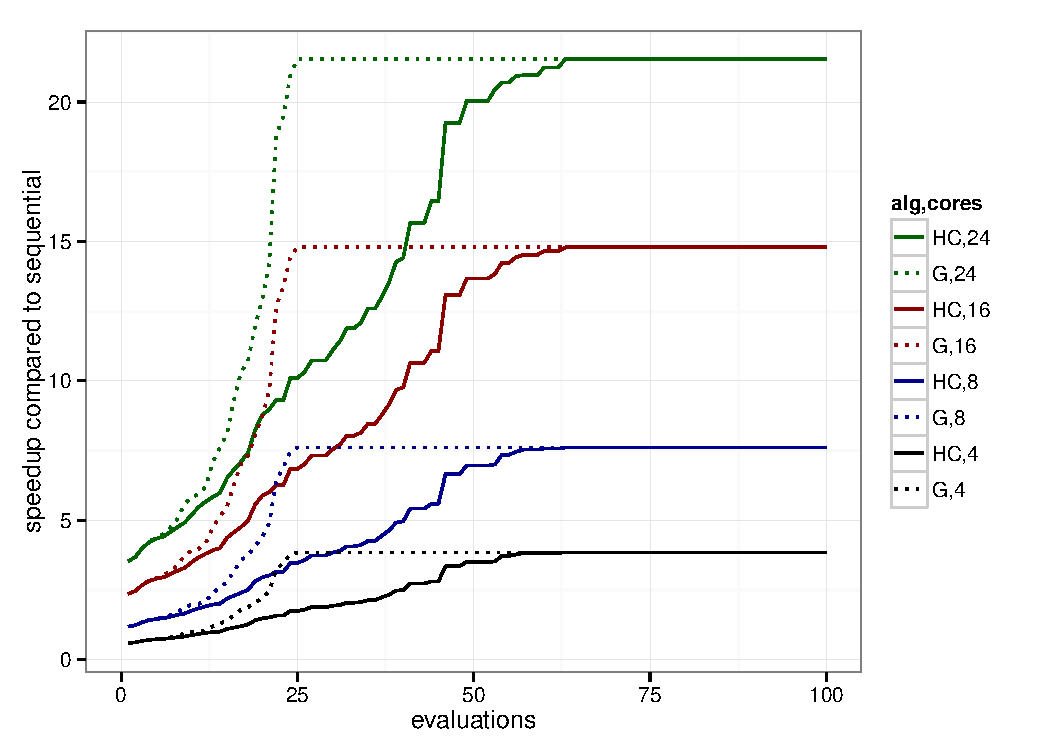
\includegraphics[scale=0.75]{Blind/Figures/speedup_by_evals_Queens2_allon_median.pdf}\\
(a) Queens2\\
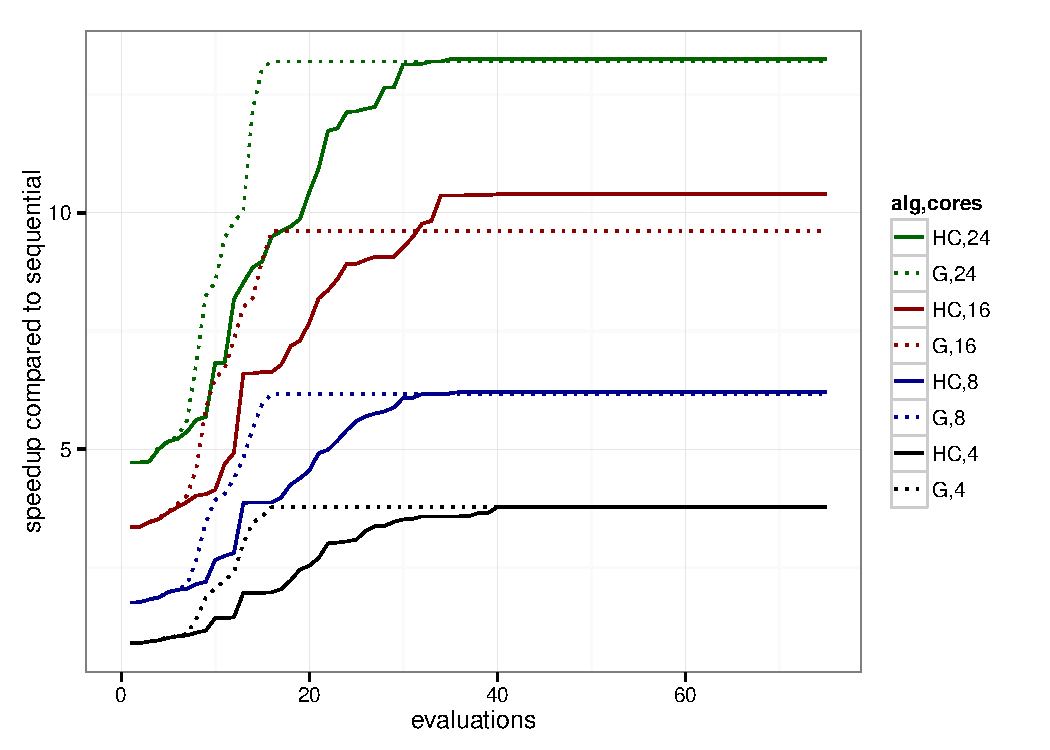
\includegraphics[scale=0.75]{Blind/Figures/speedup_by_evals_SodaCount_allon_median.pdf}\\
(b) SodaCount\\
\caption[Speedups against number of fitness evaluations for \texttt{Queens2} and \texttt{SodaCount}]{The speed-up, calculated as the ratio of the medians of the reduction counts, obtained so far by the algorithm plotted against the number of fitness evaluations. HC and G indicate the hill-climbing and greedy algorithm respectively, both using all-on initialisation. The numbers following the algorithm abbreviation indicate the number of cores.}
\label{fig:evals}
\end{figure}

\paragraph{RQ4}
For most benchmarks there is no statistically significant difference between
all-on and random initialisation.  For \verb|SodaCount|, the all-on
initialisation is slightly better for core counts of 4, 8, and 16.  This result
provides evidence that all-on initialisation may be beneficial, but requires
further investigation to confirm the generality.

\paragraph{}

The only results elided in Table \ref{tab:speedups} are the runtimes for the
greedy search with a random initialisation. This is because the random
initialisation produces inferior results in all cases and the same insight can
be gathered from studying the hill-climbing results for random initialisation.
